\documentclass[12pt]{article}

\usepackage{fullpage}
\usepackage{mdframed}
\usepackage{colonequals}
\usepackage{algpseudocode}
\usepackage{algorithm}
\usepackage{tcolorbox}
\usepackage[all]{xy}
\usepackage{proof}
\usepackage{mathtools}
\usepackage{bbm}
\usepackage{amssymb}
\usepackage{amsthm}
\usepackage{amsmath}
\usepackage{amsxtra}
\newcommand{\bb}{\mathbb}


\newtheorem{theorem}{Theorem}[section]
\newtheorem{corollary}{Corollary}[theorem]
\newtheorem{lemma}{Lemma}

\newcommand{\mathcat}[1]{\textup{\textbf{\textsf{#1}}}} % for defined terms

\newenvironment{problem}[1]
{\begin{tcolorbox}\noindent\textbf{Problem #1}.}
{\vskip 6pt \end{tcolorbox}}

\newenvironment{enumalph}
{\begin{enumerate}\renewcommand{\labelenumi}{\textnormal{(\alph{enumi})}}}
{\end{enumerate}}

\newenvironment{enumroman}
{\begin{enumerate}\renewcommand{\labelenumi}{\textnormal{(\roman{enumi})}}}
{\end{enumerate}}

\newcommand{\defi}[1]{\textsf{#1}} % for defined terms

\theoremstyle{remark}
\newtheorem*{solution}{Solution}

\setlength{\hfuzz}{4pt}

\newcommand{\calC}{\mathcal{C}}
\newcommand{\calF}{\mathcal{F}}
\newcommand{\C}{\mathbb C}
\newcommand{\N}{\mathbb N}
\newcommand{\Q}{\mathbb Q}
\newcommand{\R}{\mathbb R}
\newcommand{\Z}{\mathbb Z}
\newcommand{\F}{\mathbb F}
\newcommand{\br}{\mathbf{r}}
\newcommand{\RP}{\mathbb{RP}}
\newcommand{\CP}{\mathbb{CP}}
\newcommand{\nbit}[1]{\{0, 1\}^{#1}}
\newcommand{\bits}{\{0, 1\}^{n}}
\newcommand{\bbni}{\bigbreak \noindent}
\newcommand{\norm}[1]{\left\vert\left\vert#1\right\vert\right\vert}
\newcommand{\dbar}{\overline{\partial}}
\let\d\relax
\let\calF\relax
\newcommand{\d}{\partial}
\newcommand{\calO}{\mathcal{O}}
\newcommand{\calF}{\mathcal{F}}
\newcommand{\calG}{\mathcal{G}}
\newcommand{\calH}{\mathcal{H}}
\newcommand{\calE}{\mathcal{E}}

\let\1\relax
\newcommand{\1}{\mathbf{1}}
\newcommand{\fr}[2]{\left(\frac{#1}{#2}\right)}

\newcommand{\vecz}{\mathbf{z}}
\newcommand{\vecr}{\mathbf{r}}
\DeclareMathOperator{\Cinf}{C^{\infty}}
\DeclareMathOperator{\Id}{Id}

\DeclareMathOperator{\Alt}{Alt}
\DeclareMathOperator{\ann}{ann}
\DeclareMathOperator{\codim}{codim}
\DeclareMathOperator{\End}{End}
\DeclareMathOperator{\Hom}{Hom}
\DeclareMathOperator{\id}{id}
\DeclareMathOperator{\M}{M}
\DeclareMathOperator{\Mat}{Mat}
\DeclareMathOperator{\Ob}{Ob}
\DeclareMathOperator{\opchar}{char}
\DeclareMathOperator{\opspan}{span}
\DeclareMathOperator{\rk}{rk}
\DeclareMathOperator{\sgn}{sgn}
\DeclareMathOperator{\Sym}{Sym}
\DeclareMathOperator{\tr}{tr}
\DeclareMathOperator{\img}{img}
\DeclareMathOperator{\CandE}{CandE}
\DeclareMathOperator{\CandO}{CandO}
\DeclareMathOperator{\argmax}{argmax}
\DeclareMathOperator{\first}{first}
\DeclareMathOperator{\last}{last}
\DeclareMathOperator{\cost}{cost}
\DeclareMathOperator{\dist}{dist}
\DeclareMathOperator{\path}{path}
\DeclareMathOperator{\parent}{parent}
\DeclareMathOperator{\argmin}{argmin}
\DeclareMathOperator{\excess}{excess}
\let\Pr\relax
\DeclareMathOperator{\Pr}{\mathbf{Pr}}
\DeclareMathOperator{\Exp}{\mathbb{E}}
\DeclareMathOperator{\Var}{\mathbf{Var}}
\let\limsup\relax
\DeclareMathOperator{\limsup}{limsup}
%Paired Delims
\DeclarePairedDelimiter\ceil{\lceil}{\rceil}
\DeclarePairedDelimiter\floor{\lfloor}{ \rfloor}


\newcommand{\dagstar}{*}

\newcommand{\tbigwedge}{{\textstyle{\bigwedge}}}
\setlength{\parindent}{0pt}
\setlength{\parskip}{5pt}


\begin{document}

\title{CS 40: Computational Complexity}

\author{Sair Shaikh}
\maketitle

Collaboration Notice: Talked to Henry Scheible '26 to discuss ideas.


\begin{problab}{1}
    Suppose that $f: X \to Y$ is a homotopy equivalence. Show that the map $\pi_0(f): \pi_0(X) \to \pi_0(Y)$ from Homework 1, Problem 5 is a bijection.
\end{problab}
\begin{solu}
    Recall the map $\pi_0(f): \pi_0(X) \to \pi_0(Y)$ is defined as follows. For $[x] \in \pi_0(X)$, we have:
    \[ \pi_0(f)([x]) = [f(x)] \]
    Let $g$ be a homotopy inverse of $f$, i.e. $f \circ g \simeq \id_Y$ and $g \circ f \simeq \id_X$. First, we show that for any $x \in X$, we have $[\id_X(x)] = [g(f(x))] \in \pi_0(X)$. \\
    Let $H: X \times I \to X$ be a homotopy between $g \circ f$ and $\id_X$. Then, we note that $H(x, 0) = g(f(x))$ and $H(x, 1) = x$. Thus, $\gamma: I \to X$ defined by 
    \[ \gamma(t) = H(x, t)\]
    is a path from $g(f(x))$ to $x$ (restriction of a continous function is continous). Thus, $[g(f(x))] = [\id_X(x)]$ in $\pi_0(X)$. \\
    Thus, we conclude that $\pi_0(g \circ f) = \pi_0(\id_X)$. By the functoriality of $\pi_0$, we have that: 
    \[\pi_0(g) \circ \pi_0(f) = \id_{\pi_0(X)}\]
    Thus, $\pi_0(f)$ is injective. Similarly, we can show that $\pi_0(f) \circ \pi_0(g) = \id_{\pi_0(Y)}$, hence $\pi_0(f)$ is surjective. Thus, $\pi_0(f)$ is bijective. We can also just note that $\pi_0(f)$ is has a two-sided inverse to conclude this.
\end{solu}
\newpage

\begin{problab}{2}
    (0.11) Show that a continuous map $f: X \to Y$ is a homotopy equivalence if there exist continuous maps $g, h: Y \to X$ such that $f\circ g \simeq \id_Y$ and $h \circ f \simeq \id_X$. More generally, show that $f$ is a homotopy equivalence if $f \circ g$ and $h \circ f$ are homotopy equivalences.
\end{problab}
\begin{solu}
    Since homotopy equivalence respects composition, note that: 
    \begin{align*}
        h &= h \circ \id_Y \\
        &\simeq h \circ (f \circ g) \\
        &= (h \circ f) \circ g \\
        &\simeq \id_X \circ g \\
        &= g
    \end{align*}
    Thus, we have that $f \circ g \simeq f \circ h \simeq \id_X$. Thus $h$ is a homotopy inverse of $f$ and $f$ is a homotopy equivalence.\\
    More generally, let $f \circ g$ be a homotopy equivalance with inverse $\psi: Y \to Y$ and $h \circ f$ be a homotopy equivalence with inverse $\phi : X \to X$. Then, we have that: 
    \begin{align*}
        f \circ g \circ \psi \simeq \id_Y \\
        \phi \circ h \circ f \simeq \id_X    
    \end{align*}
    Then, let $g \circ \psi$ and $\phi \circ f$ take the role of $g$ and $h$ in the preceding argument. We conclude that $f$ is a homotopy equivalence.   
    % Let $H : Y \times I \to Y$ be a homotopy between $f \circ g$ and $\id_Y$. Consider $K: Y \times I \to X$ by $K = h \circ H$. Note that: 
    % \begin{align*}
    %     K(y, 0) &= h \circ H(y, 0) = h \circ f \circ g(y) \\
    %     K(y, 1) &= h \circ H(y, 0) = h \circ \id_Y(y) = h(y)
    % \end{align*}
    % Thus, $K$ is a homotopy between $h \circ f \circ g$ and $h$. \\
    % Similarly, let $H': X \times I \to X$ be a homotopy between $h \circ f$ and $\id_X$. Define $K': Y \times I \to X$ by $K'(y, t) = H'(g(y), t)$. Note that:
    % \begin{align*}
    %     K'(y, 0) &= H'(g(y), 0) = h \circ f \circ g(y)\\
    %     K(y, 1) &= H'(g(y), 1) = \id_X(g(y)) = g(y) 
    % \end{align*}  
    % Thus, $K'$ is a homotopy from $h \circ f \circ g$ to $g$. Since homotopy is an equivalence relation, we concluse that $g \simeq h$. Since composition respects the homotopy equivalence relation, we have that $f \circ g \simeq f \circ h \simeq \id_X$. Thus $h$ is a homotopy inverse of $f$ and $f$ is a homotopy equivalence. \\
\end{solu}
\newpage

\begin{problab}{3}
    Suppose that $G$ is a group and $G_1, \hdots, G_n$ are subgroups that generate $G$ such that $G_i \cap G_j = \{ 1 \}$ for $i \neq j$. Show that $G$ is the free product $G_1 * \hdots * G_n$ if and only if for every group $H$ and collection of homomorphisms $h_j : G_j \to H$, there exists a unique homomorphism $h: G \to H$ such that $h_j = h \circ i_j$ where $i_j: G_j \to G$ is the inclusion.
\end{problab}
\begin{solu}
    Assume $G$ is the free product $G_1 * \hdots * G_n$. Then, we know that every $g \in G$ can be written as a unique finite reduced word $g_1 \cdots g_k$, where for each $i$ there exists a unique $j$ such that $g_i \in G_j$. Moreover, we have the inclusion maps: 
    \[ \iota_j : G_j \to G \qquad \iota_j(g) = g\] 
    Now let $H$ be a group such that $h_j : G_j \to H$ are homomorphisms. We can define a map $h: G \to H$ by sending $g_1 \cdots g_k$ to $h_{j_1}(g_1) \cdots h_{j_k}(g_k)$, where $j_i$ is the unique index such that $g_i \in G_{j_i}$. It is easy to check that $h_j = h \circ \iota_j$ as for any $x \in G_j$, 
    we have: 
    \[ h \circ \iota_j(x) = h(x) = h_j(x)\]
    by definition. Next, we check that this is a homomorphism. Let $A = g_1 \cdots g_k$ and $B = g_1' \cdots g_l'$ be two reduced words in $G$. Then, we have the following cases:
    \begin{enumerate}
        \item Assume $g_k$ and $g_1'$ are in different $G_j$. Then, we have no reductions and we compute: 
        \begin{align*}
            h(A)h(B) &= h(g_1 \cdots g_k) \cdot h(g_1' \cdots g_l') \\
            &= h_{j_1}(g_1) \cdots h_{j_k}(g_k) \circ h_{i_1}(g_1') \cdots h_{i_l}(g_l') \\
            &= h(AB)
        \end{align*}
        \item Assume $g_k$ and $g_1'$ are in the same $G_j$. Then, by the reduction laws, when calculating $h(AB)$ we multiply $g_k$ and $g_1'$ first, removing it if its the identity. In calculating $h(A)h(B)$, however, the corresponding spots in the image are $h_j(g_k)h_j(g_1')$. Since $h_j$ is a homomorphism, we have that $h_j(g_k)h_j(g_1') = h_j(g_k g_1')$. Notably, if $g_k g_1' = 1$, then $h_j(g_k)h_j(g_1') = 1 \in H$ as well (as $h_j$ is a group homomorphism) and can be dropped from the expression. Thus, doing this until there are no reductions, the image $h(AB)$ with the reduction laws agrees with the image of $h(A)h(B)$ by the previous case.
    \end{enumerate}
    This can be stated more formally by inducting on the number of reductions. Thus, $h$ is a homomorphism. To show that it is unique, assume there exists another homomorphism $h': G \to H$ such that $h_j = h' \circ i_j$. Then, for each $1 \leq j \leq n$, and each $x \in G_j$, we have that: 
    \[ h(x) = h \circ \iota_j(x) = h_j(x) = h' \circ \iota_j(x) = h'(x) \]
    Thus, $h = h'$ on reduced words of length $1$. Now, assume $h = h'$ on reduced words of length $k$. Let $A = g_1 \cdots g_k \cdot g_{k+1}$ with $g_{k+1} \in G_j$. Then, we have that:
    \begin{align*}
        h(A) &= h(g_1 \cdots g_k)h(g_{k+1}) \\
        &= h'(g_1 \cdots g_k)h_{j}(g_{k+1}) \\
        &= h'(g_1 \cdots g_k)h'(g_{k+1}) \\
        &= h'(A)
    \end{align*}
    Thus, by induction, we have that $h = h'$ on all reduced words. Thus, $G$ satisfies the universal property of free products. \bbni 
    Conversely, assume that $G$ satisfies the universal property of free products. We also know that $G'$, under the definition of having a unique reduced word representation for every element, satisfies the universal property by the argument above. Moreover, we proved in class that if two groups satisfy this universal property, then they are the same group. The argument, in short, is that: Let $\phi$ be the unique homomorphism from $G$ to $G'$ and $\psi$ ber the unique homomorphism from $G'$ to $G$, given by the universal properties. Then, we have: 
    \[ \iota_{j, G'} = \phi \circ \iota_{j, G} \qquad \iota_{j, G} = \psi \circ \iota_{j, G'} \]
    Thus, we have:
    \[ \iota_{j, G'} = \phi \circ \psi \circ \iota_{j, G'} \qquad \iota_{j, G} = \phi \circ \psi \circ \iota_{j, G} \]
    However, note that $\id_G'$ and $\id_G$ satisfy the same equations, respectively. Moreover, this is the commutative equation obtained from applying the universal property of $G$ and $G'$ to themselves. Thus, the obtained homomorphisms must be unique. Thus, $\phi \circ \psi = \id_{G'}$ and $\psi \circ \phi = \id_G$. Thus, $G = G'$.
\end{solu}
\newpage

\begin{problab}{4}
    Find the fundamental group of each arrangement of three spheres below.
    \begin{enumerate}
    \item A chain. 
    \begin{center} 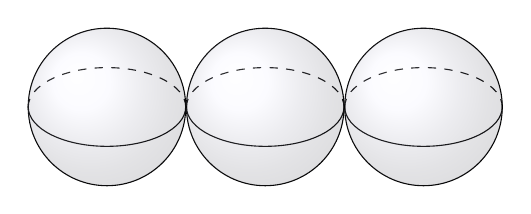
\begin{tikzpicture}
        \draw (-1,0) arc (180:360:1cm and 0.5cm);
        \draw[dashed] (-1,0) arc (180:0:1cm and 0.5cm);
        \draw (0,0) circle (1cm);
        \shade[ball color=blue!10!white,opacity=0.20] (0,0) circle (1cm);
        
        \begin{scope}[xshift = 2.01cm]
            \draw (-1,0) arc (180:360:1cm and 0.5cm);
        \draw[dashed] (-1,0) arc (180:0:1cm and 0.5cm);
        \draw (0,0) circle (1cm);
        \shade[ball color=blue!10!white,opacity=0.20] (0,0) circle (1cm);
        \end{scope}
        
        \begin{scope}[xshift = -2.01cm]
            \draw (-1,0) arc (180:360:1cm and 0.5cm);
        \draw[dashed] (-1,0) arc (180:0:1cm and 0.5cm);
        \draw (0,0) circle (1cm);
        \shade[ball color=blue!10!white,opacity=0.20] (0,0) circle (1cm);
        \end{scope}
      \end{tikzpicture}
      \end{center}
    \item A triangle.
    \begin{center} 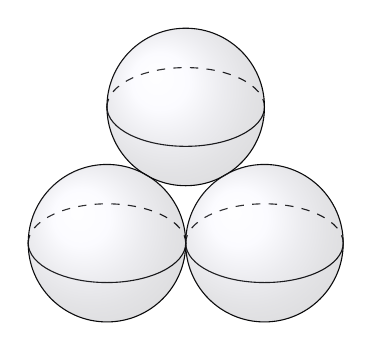
\begin{tikzpicture}
        \draw (-1,0) arc (180:360:1cm and 0.5cm);
        \draw[dashed] (-1,0) arc (180:0:1cm and 0.5cm);
        \draw (0,0) circle (1cm);
        \shade[ball color=blue!10!white,opacity=0.20] (0,0) circle (1cm);
        
        \begin{scope}[xshift = 1 cm, yshift= -1.73 cm]
            \draw (-1,0) arc (180:360:1cm and 0.5cm);
        \draw[dashed] (-1,0) arc (180:0:1cm and 0.5cm);
        \draw (0,0) circle (1cm);
        \shade[ball color=blue!10!white,opacity=0.20] (0,0) circle (1cm);
        \end{scope}
        
        \begin{scope}[xshift = -1cm, yshift=-1.73 cm]
            \draw (-1,0) arc (180:360:1cm and 0.5cm);
        \draw[dashed] (-1,0) arc (180:0:1cm and 0.5cm);
        \draw (0,0) circle (1cm);
        \shade[ball color=blue!10!white,opacity=0.20] (0,0) circle (1cm);
        \end{scope}
      \end{tikzpicture}
      \end{center}
    \end{enumerate}
\end{problab}
\begin{solu}
    Throughout this answer, contractible means deformation retractible. 
    \begin{enumerate}
        \item First, we calculate the fundamental group of the wedge of two spheres, call it $X'$. Let $U$ be the union of the two spheres minus the right-most point of the right sphere, and $V$ be the union of the two spheres minus the left-most point of the left sphere. Clearly, $U$ and $V$ are open as they are the whole space minus one point. Moreover, clearly $X' = U \cap V$. \\ 
        Next, recall that a sphere minus a point can be deformation retracted to any other point on the sphere. Note that $U \cap V$ is the union of two spheres with one point removed each, glued at a different point. Thus, $U \cap V$ is contractible to the gluing point, and is thus simply connected. Moroever, $U$ and $V$ can similarly contractible to a sphere $S^2$. Thus, we can use the Seifert van Kampen Theorem to compute the fundamental group of $X'$. We have that: 
        \[  \pi_1(X') = \pi_1(U) * \pi_1(V) = \{1\} * \{1\} = \{1\}\]
        Thus, $X'$ is simply connected. \\
        Now, we take $X$ as the gluing of $X'$ at a point (different from the gluing point of $X'$) to another sphere $S^2$ (imagine to the right). Similarly, define $U$ as the whole space minus the the right-most point of the right-most sphere, and $V$ as the whole space minus the left-most point of the left-most sphere. Clearly, $U$ and $V$ are open as they are the whole space minus one point. Moreover, clearly $X = U \cap V$. \\
        Next, not that $U \cap V$ is contractible to a sphere, which is simply connected, and $U$ and $V$ are contractible to $X'$. Thus, we can use the Seifert van Kampen Theorem to compute the fundamental group of $X$. We have that:
        \[  \pi_1(X) = \pi_1(U) * \pi_1(V) = \pi_1(X') * \pi_1(X') = \{1\} * \{1\} = \{1\}\]
        Thus, $X$ is simply connected.
        \item I'm not sure how to state this rigorously (without pictures). I would love feedback on this. \\
        Imagine the gluing points of the two spheres are along the equators, with the gluing points called $a, b, c$. Let $U$ be the whole space minus the north poles of every sphere, and $V$ be the whole space minus the south poles of every sphere. Clearly, $U$ and $V$ are open as they are the whole space minus a finite number of points. Moreover, clearly $X = U \cap V$. \bbni
        Next, consider $U \cap V$. This is the the whole space minus the north and south poles of every sphere, and thus contractible to the $3$ equator circles of each sphere glued similarly. Thus, $U \cap V$ is path-connected and we can use the Seifert van Kampen Theorem to compute the fundamental group of $X$. \bbni
        Next, note that each of the components in $U$ that come from each sphere is contractible to the arc on the equator joining the two gluing points. Thus, $U$ is contractible to the triangle containing $a, b, c$, which is homotopic to $S^1$. Similarly, $V$ is homotopic to $S^1$. Thus, 
        \[ \pi_1(U) * \pi_1(V) = \langle x, y \rangle \]
        Next, we consider loops in $\gamma = \pi_1(U \cap V)$. Note that $\gamma$ can go around the three circles in any order, and however many times. Thus, $\pi_1(U \cap V)$ is the free group $Z * Z * Z$ on three generators. However, in $U$, if $\gamma$ does one or more full loops around any of the circles, we can contract this to a the arc between the two gluing points by moving towards the South Pole. Moreover, similarly, going between the two gluing points on one arc in $U$ can be deformed into going along any other arc in $U$. Thus, the only non-trivial loops in $U$ are those generated by the loop that goes around the three circles along the boundary once (hitting all three gluing points). This loop, pushed-forward to $U$ is then the generator of $\pi_1(U)$, i.e. $x$. The same argument holds for $V$ by symmetry, thus, the push-forward of this loop to $V$ is the generator of $\pi_1(V)$, i.e. $y$. Thus, we have that:
        \[ \pi_1(X) = \pi_1(U) * \pi_1(V) = \langle x, y | xy^{-1} \rangle\]
        Finally, as $xy^{-1} = 1$ implies $x = y$, we have $\pi_1(X) = \Z$.    
    \end{enumerate}
\end{solu}
\newpage

\begin{problab}{5}
    (1.2.3) Let $X$ be the union of $n$ lines through the origin in $\R^3$. Compute the fundamental group of $\R^3 \setminus X$. 
\end{problab}
\begin{solu}
    Recall that $\R^3$ deformation retracts onto $S^2$ by the radical projection map, call it $r$. Thus, $\R^3 \setminus X$ deformation retracts onto $S^2$ minus $2n$ points, in $n$ antipodal pairs (where the $n$ lines intersect the sphere), thus has the same fundamental group. \bbni
    Note that we claimed in class that $S^2$ minus $1$ point is homeomorphic to $\R^2$ via the stereographic projection. Thus, restricting this projection to omit the remaining $2n-1$ missing points, we have that $S^2$ minus $2n$ points is homeomorphic to $\R^2$ minus $2n-1$ points. Thus, they have the same fundamental group. \bbni    
    Note that without loss of generality, we can assume that the missing $2n-1$ points are all on the $x$-axis, as translating these points can be done homeomorphically (one by one, they can be brought to the $x$-axis by a linear transformation that fixes the $x$-axis). Then, we can pick a wedge of $2n-1$ circles, with each circle going around one missing point. Then, we the space clearly deformation retracts onto the wedge of $2n-1$ circles. \bbni
    Thus, we need to calculate the fundamental group of the wedge of $k$ circles. We claim this is the free group on $k$ generators. We already know that the fundamental group of a circle is $\Z$, the free group on $1$ generator. Thus, assume the result for $<k$ circles. \bbni 
    Let $Y$ be the wedge of $k$ circles. Let $U$ be the whole space minus the right- point of the right-most circle, $V$ be the right-most circle plus a connected arc on the circle before. Clearly, $U$ and $V$ are open. Moreover, clearly $Y = U \cup V$. \bbni
    Additionally, note that $U \cap V$ is the union of connected two-arcs and is thus path-connected. Thus, we can use the Seifert van Kampen theorem to compute the fundamental group of $Y$. \bbni
    Note that $U$ is contractible to the wedge of $k-1$ circles and $V$ is contractible to a circle. Moreover, $U \cap V$ is contractible to a point. Thus, we have that: 
    \[\pi_1(Y) = \pi_1\left(\bigwedge_{i=1}^{n-1} S^1\right) * \pi_1(S^1) \]
    By the induction hypothesis, this is the free group on $k$ generators. \bbni
    Thus, finally, we have that:
    \begin{align*}
        \pi_1(\R^3 \setminus X) &= \pi_1(S^2 \setminus \{2n \text{ pts}\})\\  
        &= \pi_1(\R^2 \setminus\{2n-1 \text{ pts}\}) \\
        &= \pi_1\left(\bigwedge_{i=1}^{2n-1} S^1\right) \\
        &= \underbrace{\Z * \cdots * \Z}_{2n-1}
    \end{align*}
\end{solu}
\newpage

\end{document}